% !TEX root = ../main.tex
\chapter{Firmware and Control Implementation}

\section{Runtime State Definitions}

The firmware quantities recorded in the April 11 telemetry CSV are expressed in
centimeters, degrees, and seconds. The most important runtime states are:

\begin{align}
  d_{\text{raw,cm}}     &:\ \text{instantaneous Sharp distance estimate} \\
  d_{\text{filt,cm}}    &:\ \text{filtered distance used for control} \\
  x_{\text{cm}}         &= d_{\text{filt,cm}} - d_{\text{setpoint,cm}} \\
  \dot{x}_{\text{cm/s}} &:\ \text{filtered ball-velocity estimate} \\
  \theta_{\text{cal,deg}} &:\ \text{calibrated beam angle before balance zeroing} \\
  \theta_{\text{rel,deg}} &:\ \theta_{\text{cal,deg}} - \theta_{\text{balance,deg}} \\
  \dot{\theta}_{\text{deg/s}} &:\ \text{filtered beam-angle rate estimate} \\
  \xi_{\text{cm.s}} &:\ \text{outer-loop integral state}
\end{align}

\section{Sensing and Signal Conditioning}

\subsection{Sharp Distance Sensor}

At each \SI{40}{ms} cycle the controller averages eight ADC samples and applies the
inverse-voltage fit

\begin{equation}
  d_{\text{raw,cm}} = \frac{12.25}{V_{\text{sharp}}} - 0.62
\end{equation}

with the validity limits

\begin{equation}
  V_{\text{sharp}} \ge \SI{0.08}{V},
  \qquad
  \SI{4.40}{cm} \le d_{\text{raw,cm}} \le \SI{12.66}{cm}
\end{equation}

Accepted samples pass through a three-sample median and two exponential filters:

\begin{align}
  m[k] &= \text{median of last three valid distance samples} \\
  d_{\text{filt}}[k] &= 0.25\,m[k] + 0.75\,d_{\text{filt}}[k-1] \\
  d_{\text{vel}}[k] &= 0.60\,m[k] + 0.40\,d_{\text{vel}}[k-1] \\
  d_{\text{rate}}[k] &= \frac{d_{\text{vel}}[k] - d_{\text{vel}}[k-1]}{0.04}
\end{align}

The ball-velocity estimate is then formed with adaptive smoothing so the near-sensor
side receives extra filtering.

\subsection{AS5600 Beam Angle}

The beam-angle conversion used online is the affine fit

\begin{equation}
  \theta_{\text{cal,deg}}
  = 0.07666806 \cdot \theta_{\text{AS5600,deg}} - 23.28443907
\end{equation}

The balance-zero command sets $\theta_{\text{balance,deg}}$ so that
$\theta_{\text{rel,deg}} = 0$ corresponds to the chosen control reference rather than
the raw iPhone-level zero from the calibration session.

\section{Mode Structure}

The staged firmware in \path{src/main.cpp} provides:

\begin{itemize}
  \item \textbf{M0}: telemetry only, no control output,
  \item \textbf{M1}: manual beam-angle hold with the inner loop only, and
  \item \textbf{M2}: cascaded ball-position control.
\end{itemize}

The driver starts disabled at boot. The operator enables it explicitly, captures the
balance reference with the \verb|Z| command, and then enters the cascaded mode. This
staged flow reduces risk while tuning the hardware.

\section{Implemented Cascade}

\begin{figure}[tbp]
  \centering
  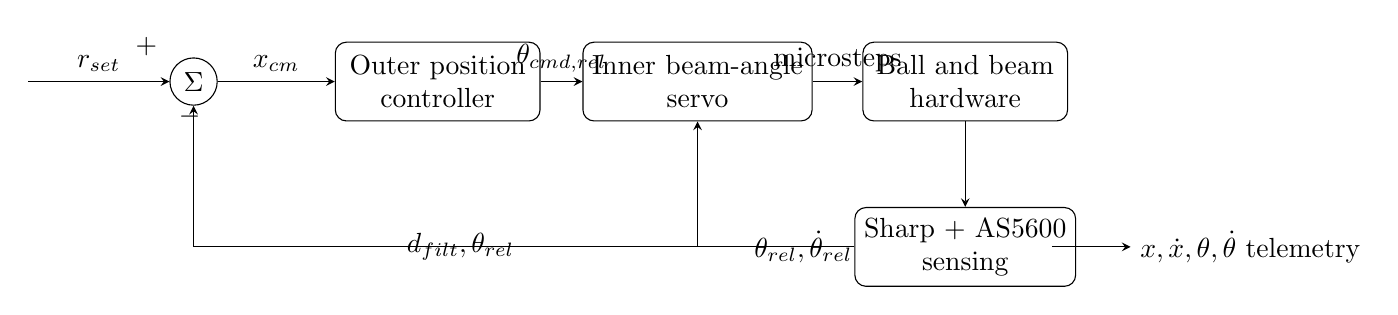
\begin{tikzpicture}[
    block/.style={draw, rounded corners, minimum width=2.6cm, minimum height=1cm, align=center},
    sum/.style={draw, circle, inner sep=0pt, minimum size=6mm},
    > = stealth
  ]
    \node[sum] (sum1) at (0,0) {$\Sigma$};
    \node[block] (outer) at (3.1,0) {Outer position\\controller};
    \node[block] (inner) at (6.4,0) {Inner beam-angle\\servo};
    \node[block] (plant) at (9.8,0) {Ball and beam\\hardware};
    \node[block] (sensorx) at (9.8,-2.1) {Sharp + AS5600\\sensing};

    \draw[->] (-2.1,0) -- node[above] {$r_{\text{set}}$} (sum1);
    \draw[->] (sum1) -- node[above] {$x_{\text{cm}}$} (outer);
    \draw[->] (outer) -- node[above] {$\theta_{\text{cmd,rel}}$} (inner);
    \draw[->] (inner) -- node[above] {microsteps} (plant);
    \draw[->] (plant) -- (sensorx);
    \draw[->] (sensorx.west) -| node[pos=0.25,left] {$d_{\text{filt}},\theta_{\text{rel}}$} (sum1.south);
    \draw[->] (sensorx.west) -| node[pos=0.35,right] {$\theta_{\text{rel}},\dot{\theta}_{\text{rel}}$} (inner.south);
    \draw[->] (10.9,-2.1) -- ++(1.0,0) node[right] {$x,\dot{x},\theta,\dot{\theta}$ telemetry};
    \node at (-0.6,0.45) {$+$};
    \node at (-0.05,-0.45) {$-$};
  \end{tikzpicture}
  \caption{Implementation-oriented cascaded control structure used by the April 11
  telemetry run.}
  \label{fig:cascade_block}
\end{figure}

\subsection{Inner Beam-Angle Servo}

The commanded beam angle is first limited to the calibrated soft window
$[-0.90,\ 3.30]$ degrees around the balance reference. The beam-angle error is

\begin{equation}
  e_{\theta,\text{deg}} = \theta_{\text{cmd,cal,deg}} - \theta_{\text{cal,deg}}
\end{equation}

If both the angle error and beam-rate magnitude are inside the deadband,
$|e_{\theta}| \le \SI{0.040}{deg}$ and
$|\dot{\theta}_{\text{deg/s}}| \le \SI{0.60}{deg/s}$, the controller outputs zero
steps. Otherwise the discrete servo computes

\begin{equation}
  \text{raw\_steps}[k] =
  -\left(0.70\,e_{\theta,\text{deg}}[k]\right)\cdot 115.9399
  + \text{residual}[k-1]
\end{equation}

and rounds the result to an integer command clipped to $\pm 40$ microsteps per cycle.

\subsection{Outer Ball-Position Law}

The outer loop clamps the derivative states to

\begin{equation}
  |x_{\dot{\text{cm/s}}}| \le \SI{4.50}{cm/s},
  \qquad
  |\theta_{\dot{\text{deg/s}}}| \le \SI{4.0}{deg/s}
\end{equation}

and then applies the tuned state-feedback law

\begin{equation}
  \theta_{\text{fs,cmd,deg}}
  = g_{\text{outer\_sign}}
    \left(
      k_x x_{\text{cm}}
      + k_v x_{\dot{\text{cm/s}}}
      + k_t \theta_{\text{rel,deg}}
      + k_{\omega} \theta_{\dot{\text{deg/s}}}
      + i_{\text{term,deg}}
    \right)
\end{equation}

with the April 11 defaults

\begin{align}
  g_{\text{outer\_sign}} &= -1 \\
  k_x &= 0.28 \\
  k_v &= 0.20 \\
  k_t &= 0.00 \\
  k_{\omega} &= 0.00 \\
  k_i &= 0.020
\end{align}

The integral state is constrained to the near-target capture region and clipped so that
$|i_{\text{term,deg}}| \le \SI{0.18}{deg}$.

\subsection{Recovery and Trim Logic}

The implementation retains three important practical features:

\begin{itemize}
  \item a \textbf{recovery floor} that enforces a minimum corrective beam command when
  the ball appears stalled away from the setpoint,
  \item a \textbf{zero-trim estimator} that logs a slow local balance-angle estimate
  under tight near-equilibrium conditions, and
  \item a \textbf{position-trim map} that can learn a local hold-angle bias across the
  usable setpoint range.
\end{itemize}

No learned position-trim feedforward was active during the April 11 run, so the
telemetry shows \verb|theta_trim_ff_deg = 0| for every row.

\section{Implementation Constants}

Table~\ref{tab:implementation_constants} compresses the runtime constants most relevant
to reproducing the telemetry run.

\small
\begin{longtable}{@{}p{0.19\linewidth}p{0.27\linewidth}p{0.14\linewidth}p{0.30\linewidth}@{}}
\caption{Key runtime constants from the firmware implementation in \texttt{src/main.cpp}.}
\label{tab:implementation_constants}\\
\toprule
Group & Constants & Value & Meaning \\
\midrule
\endfirsthead
\toprule
Group & Constants & Value & Meaning \\
\midrule
\endhead
\bottomrule
\endfoot
Timing & \verb|LOOP_MS|, \verb|DT| & \SI{40}{ms}, \SI{0.040}{s} & Main control cadence \\
Distance window & \verb|D_MIN_CM|, \verb|D_MAX_CM|, \verb|D_SETPOINT_DEFAULT_CM| & \SI{4.40}{cm}, \SI{12.66}{cm}, \SI{8.53}{cm} & Allowed sensing and default center setpoint \\
Sharp fit & \verb|SHARP_FIT_K_V_CM|, \verb|SHARP_FIT_OFFSET_CM| & 12.25, -0.62 & Inverse-voltage distance calibration \\
Angle calibration & \verb|THETA_SLOPE_DEG_PER_AS_DEG|, \verb|THETA_OFFSET_DEG| & 0.07666806, -23.28443907 & Online AS5600 to beam-angle affine fit \\
Angle limits & \verb|THETA_CAL_MIN_DEG|, \verb|THETA_CAL_MAX_DEG| & -0.70, 3.10 & Measured calibrated beam-angle range \\
Stepper conversion & \verb|STEPS_PER_REV|, \verb|STEPS_PER_BEAM_DEG| & 3200, 115.9399 & Empirical beam-angle to microstep conversion \\
Inner loop & \verb|INNER_KP_THETA|, \verb|INNER_KD_THETA|, \verb|INNER_MAX_STEP_DELTA| & 0.70, 0.00, 40 & Discrete beam-angle servo gains and step clamp \\
Outer loop & \verb|OUTER_KX_DEFAULT|, \verb|OUTER_KV_DEFAULT|, \verb|OUTER_KI_DEFAULT| & 0.28, 0.20, 0.020 & Default position-feedback and integral gains \\
Recovery & \verb|RECOVERY_ENTER_X_CM|, \verb|RECOVERY_FLOOR_DEFAULT_DEG|, \verb|RECOVERY_FLOOR_MAX_DEG| & \SI{1.20}{cm}, \SI{0.70}{deg}, \SI{1.10}{deg} & Stall detection and minimum corrective angle floor \\
Staircase & \verb|STAIRCASE_STAGE_MS|, \verb|STAIRCASE_FAR_SETPOINT_CM|, \verb|STAIRCASE_CENTER_SETPOINT_CM|, \verb|STAIRCASE_NEAR_SETPOINT_CM| & \SI{20000}{ms}, 12.16, 8.53, 4.90 & Built-in experiment sequence used in the telemetry log \\
\end{longtable}
\normalsize
